% Borrador del reporte final en español (formato IEEE Conference, dos columnas).
% Las limitaciones (sin noches frias, sin medicion de consumo) se dicen en el texto.
% IMPORTANTE: es un borrador de trabajo. Cada integrante debe leerlo, corregirlo
% y reescribirlo con sus palabras antes de entregarlo.
% Nota: los lineamientos piden el reporte final en ingles; esta version en espanol
% sirve para organizar el contenido y despues traducirlo.
\documentclass[conference]{IEEEtran}
\IEEEoverridecommandlockouts
\usepackage[utf8]{inputenc}
\usepackage[T1]{fontenc}
\usepackage[spanish,es-nodecimaldot]{babel}
\usepackage{cite}
\usepackage{amsmath}
\usepackage{graphicx}
\usepackage{booktabs}
\usepackage{array}
\usepackage{xcolor}
\usepackage{tikz}
\usetikzlibrary{positioning,arrows.meta,fit}
\usepackage{url}
\def\UrlBreaks{\do\/\do-\do.\do_}
\addto\captionsspanish{\renewcommand{\tablename}{Tabla}}
\newcommand{\pend}[1]{\textcolor{red!70!black}{\textbf{[PENDIENTE: #1]}}}
\begin{document}

\title{Nodo TinyML de bajo costo para la clasificaci\'on local del riesgo de helada y la validaci\'on de pron\'osticos en la vereda Pirgua, Tunja\\
{\large Reporte final}}

\author{\IEEEauthorblockN{Mateo \'Avila Romero}
\IEEEauthorblockA{\textit{Ingenier\'ia de Datos e Inteligencia Artificial}\\
\textit{Universidad Santo Tom\'as}, Tunja, Colombia}
\and
\IEEEauthorblockN{Andres Mateo Carvajal Ricon}
\IEEEauthorblockA{\textit{Ingenier\'ia de Datos e Inteligencia Artificial}\\
\textit{Universidad Santo Tom\'as}, Tunja, Colombia}
\and
\IEEEauthorblockN{Johan Mahomer Leon Beltran}
\IEEEauthorblockA{\textit{Ingenier\'ia de Datos e Inteligencia Artificial}\\
\textit{Universidad Santo Tom\'as}, Tunja, Colombia}}

\maketitle

\begin{abstract}
Las heladas da\~nan los cultivos de papa y los pastos del altiplano de Boyac\'a, y los pron\'osticos regionales no describen el microclima de cada predio. Este reporte describe un nodo embebido de bajo costo instalado en la vereda Pirgua (Tunja). Un ESP32-S3 lee un sensor BME280 y est\'a dise\~nado para clasificar el riesgo de helada en el propio dispositivo con un modelo TensorFlow Lite Micro cuantizado a int8, a partir de una ventana de 3 horas guardada en un buffer circular. Un m\'odulo en Python extrae el pron\'ostico web de Tunja, lo guarda en una tabla hash propia y lo compara con la predicci\'on del nodo en un tablero. Presentamos la arquitectura, el protocolo de captura, un conjunto de datos propio de dos noches v\'alidas (296 lecturas, la sonda nunca por debajo de 12,4\,$^\circ$C y el BME280 nunca por debajo de 11,45\,$^\circ$C), el desfase medido entre el BME280 y una sonda de referencia, y el uso de recursos del modelo en el ESP32-S3, comparado con una Raspberry Pi Pico. Entrenamos un modelo de tres clases solo con datos p\'ublicos: en la prueba, el F1 promedio fue 0,678 en punto flotante y 0,683 en int8. Cargado en el ESP32-S3, el modelo dio la misma clase que el PC en 100 de 100 vectores de prueba y en 50 de 50 ventanas crudas, con una latencia de 0,053\,ms por inferencia. Como el conjunto propio no tiene noches fr\'ias, ese resultado no se valid\'o con datos de Pirgua, y el consumo de energ\'ia no se midi\'o.
\end{abstract}

\begin{IEEEkeywords}
computaci\'on en el borde, TinyML, TensorFlow Lite Micro, predicci\'on de heladas, web scraping, estructuras de datos
\end{IEEEkeywords}

\section{Introducci\'on}
La helada radiativa ocurre en noches despejadas y en calma, cuando el suelo y el aire cercano pierden calor r\'apidamente, y da\~na los cultivos cuando la temperatura del aire se acerca o baja de 0\,$^\circ$C \cite{fao_frost}. En el altiplano cundiboyacense, entre unos 2\,600 y 3\,000\,m, estos eventos afectan la papa, las hortalizas y los pastos. Quienes cultivan en la vereda Pirgua (Tunja) suelen enterarse de una helada cuando el da\~no ya ocurri\'o, porque los pron\'osticos se emiten por municipio y la estaci\'on oficial m\'as cercana puede estar a kil\'ometros del lote y a otra altitud.

Seg\'un el IDEAM y la UPRA, 173\,150\,ha de Boyac\'a estuvieron bajo amenaza de helada en la \'ultima semana de enero de 2024, y las 18 municipalidades de Boyac\'a con papa listadas en el informe suman cerca de 1\,368\,ha vulnerables \cite{upra2024}. En la semana del 8 al 14 de febrero de 2020 subi\'o el precio mayorista de la papa criolla porque hab\'ia menos cultivos en etapa productiva y algunos en floraci\'on resultaron da\~nados por heladas \cite{dane2020}.

La estaci\'on IDEAM UPTC Tunja (c\'odigo 2401500086) no registr\'o ninguna lectura horaria de 0\,$^\circ$C o menos entre marzo de 2019 y noviembre de 2026; su lectura m\'as fr\'ia fue 0,1\,$^\circ$C y el percentil 1 del m\'inimo diario es 3,1\,$^\circ$C \cite{ideam_data}. La serie tiene vac\'ios (cerca del 63\,\% de las horas tienen datos), de modo que una noche m\'as fr\'ia puede faltar. Nuestra hip\'otesis es que un lote en Pirgua es m\'as fr\'io que esa estaci\'on y por eso hay que medir en el sitio. Todav\'ia no hemos podido ponerla a prueba, porque las noches medidas hasta ahora fueron templadas.

\textbf{Objetivo.} Construir un nodo de bajo costo que clasifique el riesgo de helada en el propio dispositivo y validar su predicci\'on frente a un pron\'ostico web, usando solo la memoria, el c\'omputo y la energ\'ia que realmente necesita.

\textbf{Aportes.} (i) Un nodo funcional con inferencia en el borde; (ii) un protocolo de captura y un conjunto de datos propio con versiones; (iii) dos estructuras de datos escritas sin librer\'ias, con su an\'alisis de complejidad; (iv) un m\'odulo de scraping y un tablero de comparaci\'on; (v) un reporte de recursos del dispositivo frente a una placa m\'as limitada.

\section{Trabajo relacionado}
Diedrichs \textit{et al.} predijeron eventos de helada con modelos de aprendizaje autom\'atico entrenados con datos de dispositivos IoT instalados en campo \cite{diedrichs2018}. Calder\'on Caro \textit{et al.} publicaron un conjunto de datos a 30 minutos de 23 estaciones agr\'icolas del altiplano cundiboyacense con etiquetas de helada \cite{calderon2026,zenodo2026}. TensorFlow Lite Micro ejecuta redes neuronales en microcontroladores con pocos kilobytes de memoria \cite{david2021}, y la cuantizaci\'on entera reduce el tama\~no del modelo manteniendo una exactitud cercana a la del modelo en punto flotante \cite{jacob2018}. Medir TinyML exige m\'etricas consistentes de latencia, memoria y energ\'ia \cite{banbury2020}.

Esos trabajos predicen la helada en un servidor o estudian TinyML en general. Aqu\'i la clasificaci\'on corre en el propio nodo, en una vereda concreta, se documenta el consumo de recursos frente a una placa m\'as peque\~na y cada predicci\'on local se compara con el pron\'ostico p\'ublico.

\section{Arquitectura del sistema}
La Fig.~\ref{fig:block} muestra la arquitectura. El nodo lee el BME280 cada 5\,min. Las lecturas se promedian en pasos de 30\,min y se guardan en un buffer circular de 6 pasos (3\,h). Cuando el buffer est\'a lleno, el nodo calcula el punto de roc\'io con la f\'ormula de Magnus \cite{alduchov1996}, codifica la hora del d\'ia como seno y coseno, cuantiza la entrada y ejecuta el modelo. Cada lectura y cada predicci\'on se guardan en la memoria flash (LittleFS) y se imprimen por el puerto serie. En un PC, un receptor guarda las predicciones, un scraper guarda el pron\'ostico en una tabla hash cada 60\,min y un tablero en Streamlit muestra las coincidencias y las diferencias.

\begin{figure}[t]
\centering
\begin{tikzpicture}[font=\scriptsize, node distance=3mm and 4mm,
 blk/.style={draw, rounded corners=2pt, align=center, minimum height=6mm, inner sep=2pt},
 arr/.style={-{Stealth[length=2mm]}}]
\node[blk] (bme) {BME280\\T, HR, P};
\node[blk, below=of bme] (ina) {INA219\\consumo};
\node[blk, below=of ina] (ds) {DS18B20\\referencia};
\node[blk, right=9mm of ina, minimum width=28mm, minimum height=26mm] (esp) {};
\node[anchor=north, font=\scriptsize\bfseries] at (esp.north) {ESP32-S3};
\node[blk, fill=gray!10] at ([yshift=3mm]esp.center) (buf) {Buffer circular\\6 pasos $\times$ 30 min};
\node[blk, fill=gray!10, below=2mm of buf] (tfl) {TFLite Micro\\modelo int8};
\node[blk, right=7mm of esp, minimum width=22mm] (pc) {PC: receptor,\\comparaci\'on,\\tablero};
\node[blk, above=4mm of pc] (web) {P\'agina del pron\'ostico\\(cada hora)};
\node[blk, below=4mm of pc, fill=gray!10] (hash) {Tabla hash\\(municipio, hora)};
\draw[arr] (bme.east) -- node[above]{I2C} ([yshift=8mm]esp.west);
\draw[arr] (ina.east) -- node[above]{I2C} (esp.west);
\draw[arr] (ds.east) -- node[above, font=\tiny]{1-Wire} ([yshift=-8mm]esp.west);
\draw[arr] (esp.east) -- node[above]{USB} (pc.west);
\draw[arr] (web) -- (pc);
\draw[arr] (pc) -- (hash);
\end{tikzpicture}
\caption{Diagrama de bloques. La inferencia corre en el ESP32-S3; el PC solo guarda, extrae y muestra.}
\label{fig:block}
\end{figure}

\begin{figure}[t]
\centering
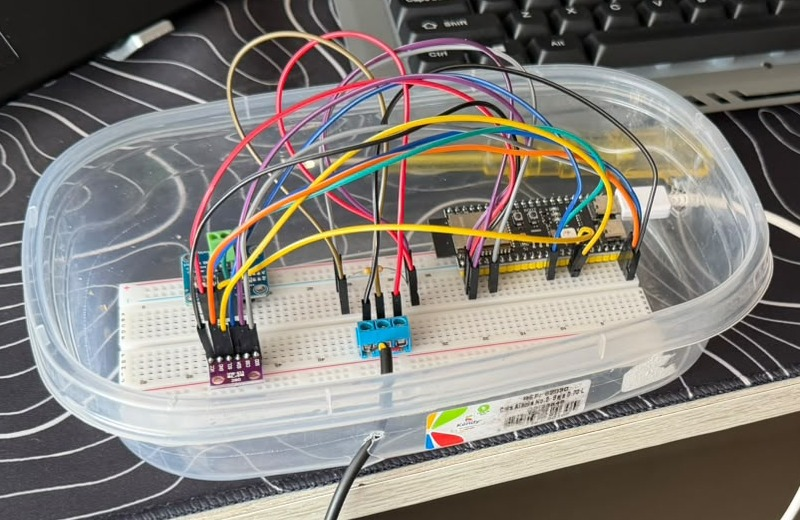
\includegraphics[width=0.85\columnwidth]{nodo.jpg}
\caption{Prototipo del nodo en protoboard dentro de su caja: ESP32-S3 y sensores.}
\label{fig:nodo}
\end{figure}

\section{Firmware y preprocesamiento}
El programa del nodo est\'a escrito para el entorno Arduino-ESP32 y ejecuta el modelo con TensorFlow Lite Micro. Cada 5 minutos despierta el BME280 en modo forzado, lee temperatura, humedad y presi\'on, y la sonda DS18B20, y guarda una fila en la memoria flash. Cuando se cierra un paso de 30 minutos, promedia las lecturas del paso y lo empuja al buffer circular. Cuando el buffer tiene sus 6 pasos, arma el vector de entrada y ejecuta una inferencia.

El punto de roc\'io $T_d$ se calcula con la aproximaci\'on de Magnus \cite{alduchov1996},
\begin{equation}
\gamma = \ln\frac{HR}{100} + \frac{aT}{b+T}, \qquad T_d = \frac{b\,\gamma}{a-\gamma},
\end{equation}
con $a=17{,}625$ y $b=243{,}04\,^\circ$C, la misma f\'ormula en el script de preparaci\'on de datos y en el firmware. Una prueba compara las dos implementaciones: con 50 ventanas crudas y el modelo final, el nodo dio la misma clase que el PC en las 50, y la misma salida int8 exacta en 48 (en las otras dos, la mayor diferencia fue de 2 unidades).

El nodo acepta comandos por el puerto serie: \texttt{STATUS}, \texttt{DUMP} (descarga el registro), \texttt{BENCHMARK} (200 inferencias y reporte de recursos), \texttt{VECTOR} (ejecuta el modelo sobre una entrada int8 cruda) y \texttt{WINDOW} (ejecuta todo el preprocesamiento y el modelo sobre lecturas crudas, sin guardar nada). Los dos \'ultimos permiten validar el modelo y el preprocesamiento por separado.

\section{Selecci\'on del dispositivo}
El dispositivo es una ESP32-S3 DevKitC-1 (m\'odulo ESP32-S3-N16R8): dos n\'ucleos Xtensa LX7 de hasta 240\,MHz con instrucciones vectoriales, 512\,KB de SRAM, 8\,MB de PSRAM, 16\,MB de flash y Wi-Fi integrado \cite{esp32s3}. Se adopt\'o por recomendaci\'on del docente del curso, y el reporte de recursos mide cu\'anto de ella usa realmente la tarea. El BME280 y el INA219 comparten un bus I2C (GPIO8 y GPIO9, direcciones 0x76 y 0x40) \cite{bme280}. Una sonda DS18B20 en GPIO4 da una temperatura de referencia que solo se usa para calibrar y no es entrada del modelo. El INA219 est\'a conectado al bus I2C para medir el consumo, pero esa medici\'on no se hizo en este trabajo.

Como alternativa m\'as limitada tomamos una Raspberry Pi Pico (RP2040: dos n\'ucleos Cortex-M0+, 264\,KB de SRAM, 2\,MB de flash, sin Wi-Fi) \cite{rp2040}. Ejecuta el mismo modelo int8 y el mismo benchmark, de modo que los dos reportes se pueden poner lado a lado. Hay adem\'as una raz\'on funcional a favor de la ESP32-S3: la Pico no tiene Wi-Fi, as\'i que no puede recuperar su reloj por NTP despu\'es de un corte de energ\'ia, y el modelo usa la hora del d\'ia como entrada.

\section{Adquisici\'on de datos}
El BME280 trabaja en modo forzado, con sobremuestreo $\times$1 y filtro apagado, de modo que duerme entre lecturas y no se calienta. Las lecturas fuera del rango de la hoja de datos se guardan con estado \texttt{sensor\_error} y se excluyen despu\'es. La Tabla~\ref{tab:protocolo} resume el protocolo.

\begin{table}[t]
\caption{Protocolo de captura}
\label{tab:protocolo}
\centering
\begin{tabular}{@{}>{\raggedright}p{2.2cm}>{\raggedright\arraybackslash}p{5.6cm}@{}}
\toprule
Par\'ametro & Valor \\
\midrule
Sitio & Vereda Pirgua, Tunja; 1,5\,m sobre el suelo, con protecci\'on solar \\
Sensores & BME280 y DS18B20 juntos, fuera de la caja, a 20--30\,cm de ella \\
Periodo & Noviembre a febrero \\
Muestreo & Cada 5\,min; promedio en pasos de 30\,min \\
Fila guardada & hora (UTC$-$5), T, HR, P, T de referencia, estado \\
Reloj & NTP por Wi-Fi en cada arranque \\
Etiqueta & m\'inimo de T de las pr\'oximas 6\,h frente a umbrales \\
Partici\'on & 70/15/15 por d\'ias completos, semilla fija \\
Versiones & v1, v2, \dots; nunca se sobrescriben \\
\bottomrule
\end{tabular}
\end{table}

\textbf{Lecci\'on de la primera noche.} La noche del 20 al 21 de noviembre el nodo funcion\'o unas 14 horas sin PC: 170 lecturas, todas v\'alidas, una cada 5 minutos y sin reinicios. Pero el BME280 estaba dentro de la caja electr\'onica y solo la sonda estaba afuera. De noche el BME280 marc\'o en promedio 4,4\,$^\circ$C m\'as que la sonda y casi no baj\'o, mientras la sonda lleg\'o a 12,5\,$^\circ$C a las 06:14. Esa noche se descart\'o del conjunto de datos y qued\'o la regla de que el BME280 mide aire exterior, nunca el de la caja.

\textbf{Calibraci\'on en sitio.} No hicimos una prueba de calibraci\'on aparte antes de la captura: el BME280 y la sonda van juntos en la protecci\'on solar, as\'i que cada lectura compara los dos sensores. El desfase (BME280 menos sonda) se calcula despu\'es de cada noche. Limitaci\'on: la sonda misma no est\'a verificada contra una temperatura conocida; el desfase dice cu\'anto difieren los sensores, no cu\'al tiene la raz\'on.

\section{Conjunto de datos y etiquetado}
\textbf{Fuentes.} El conjunto principal es el capturado con nuestro nodo. Como apoyo se usan dos fuentes p\'ublicas: la serie horaria de la estaci\'on IDEAM UPTC Tunja \cite{ideam_data} y el conjunto del altiplano \cite{zenodo2026}, con la estaci\'on 11 excluida de antemano. El conjunto del altiplano no incluye presi\'on, as\'i que si se usa para entrenar, el modelo se entrena sin esa variable. Auditamos los archivos del IDEAM: hay 3\,482 marcas de tiempo duplicadas por archivo (siempre con el mismo valor), 41\,902 horas con las tres variables a la vez y vac\'ios largos, el mayor de 537 d\'ias (marzo de 2023 a septiembre de 2024).

\begin{table}[t]
\caption{Cobertura anual de la temperatura de la estaci\'on IDEAM UPTC Tunja}
\label{tab:cob}
\centering
\footnotesize\setlength{\tabcolsep}{2.5pt}
\begin{tabular}{@{}lcccccccc@{}}
\toprule
A\~no & 2019 & 2020 & 2021 & 2022 & 2023 & 2024 & 2025 & 2026 \\
\midrule
Con dato (\%) & 95 & 93 & 69 & 45 & 16 & 18 & 84 & 91 \\
\bottomrule
\end{tabular}
\end{table}

\textbf{Rejilla y ventanas.} Todas las fuentes se promedian en una rejilla de 30\,min. Los vac\'ios se rellenan por interpolaci\'on lineal solo si las lecturas reales a cada lado distan 60\,min o menos. El IDEAM es horario, as\'i que cerca de la mitad de sus valores a 30\,min son interpolados. Cada ventana usa las 3\,h anteriores (6 pasos) para predecir el m\'inimo de las 6\,h siguientes.

\textbf{Clases.} Decidimos tres clases a partir del m\'inimo de las pr\'oximas 6\,h (Tabla~\ref{tab:clases}). El l\'imite de 2\,$^\circ$C se justifica porque los sensores est\'an a 1,5\,m y en noches despejadas la superficie del cultivo puede estar varios grados m\'as fr\'ia que el aire a esa altura \cite{fao_frost}. El l\'imite de 6\,$^\circ$C es una banda operativa y no un valor agron\'omico: da al modelo ejemplos de noches fr\'ias, porque las de 2\,$^\circ$C o menos son raras (en la serie del IDEAM hay 9 d\'ias entre 2019 y 2026). Ambos valores son par\'ametros y cambiarlos exige construir una nueva versi\'on del conjunto. Como referencia agron\'omica, la FAO lista para la papa temperaturas cr\'iticas de $-1$ a $-2$\,$^\circ$C en floraci\'on y fructificaci\'on, y de $-2$ a $-3$\,$^\circ$C en germinaci\'on (Tabla~4.5 del cap\'itulo~4, tomada de Ventskevich, 1958) \cite{fao_frost}. El cap\'itulo no aclara si son temperaturas del aire o de la hoja, ni la duraci\'on, y las presenta solo como gu\'ia. No encontramos un umbral oficial de Fedepapa o del ICA para el aire a 1,5\,m.

\begin{table}[t]
\caption{Clases de riesgo}
\label{tab:clases}
\centering
\begin{tabular}{@{}clc@{}}
\toprule
Clase & Nombre & M\'inimo de las pr\'oximas 6\,h \\
\midrule
0 & sin riesgo & mayor que 6\,$^\circ$C \\
1 & precauci\'on & mayor que 2 y hasta 6\,$^\circ$C \\
2 & riesgo & hasta 2\,$^\circ$C \\
\bottomrule
\end{tabular}
\end{table}

\textbf{Partici\'on sin fuga.} La partici\'on es por d\'ias calendario completos (70/15/15\,\%), con semilla fija: todas las lecturas de un d\'ia quedan en el mismo conjunto, y un d\'ia queda en el mismo conjunto para todas las fuentes. Est\'a estratificada por la clase m\'as alta de cada d\'ia, para que los d\'ias fr\'ios, que son raros, lleguen tambi\'en a validaci\'on y prueba. Una ventana cercana a la medianoche usa unas horas del d\'ia vecino; es una limitaci\'on conocida.

\textbf{Composici\'on de la versi\'on 1.} La Tabla~\ref{tab:v1} muestra la versi\'on 1: 699\,850 ventanas de 3\,h. Los ejemplos fr\'ios vienen de las fuentes p\'ublicas. El conjunto propio aporta 17 ventanas de 3 d\'ias, todas de clase 0, y ninguna cae en el conjunto de prueba. Por eso, hoy, ning\'un resultado del modelo puede apoyarse en datos propios.

\begin{table}[t]
\caption{Ventanas de la versi\'on 1 por fuente y clase}
\label{tab:v1}
\centering
\begin{tabular}{@{}lrrrr@{}}
\toprule
Fuente & Clase 0 & Clase 1 & Clase 2 & Total \\
\midrule
Nodo (Pirgua) & 17 & 0 & 0 & 17 \\
IDEAM UPTC & 78\,234 & 2\,660 & 114 & 81\,008 \\
Altiplano & 557\,692 & 54\,481 & 6\,652 & 618\,825 \\
\bottomrule
\end{tabular}
\end{table}

\section{Estructuras de datos}
Escribimos dos estructuras sin librer\'ias (Tabla~\ref{tab:ds}).

\textbf{Buffer circular (borde).} El modelo necesita las lecturas de las \'ultimas 3 horas: 6 pasos de 30 minutos. Cada 30 minutos llega un paso nuevo y el m\'as viejo deja de servir. Usamos un arreglo fijo de $n=6$ posiciones y un \'indice \texttt{head} que vuelve a 0 despu\'es de la \'ultima posici\'on; cuando est\'a lleno, el nuevo dato sobrescribe al m\'as viejo. Un arreglo que desplaza todos los datos en cada inserci\'on cuesta $O(n)$, y una lista enlazada necesita memoria din\'amica, que en un microcontrolador puede fragmentar el heap. Con $n=6$ la diferencia de tiempo es peque\~na, pero el buffer circular tiene un costo constante y conocido y no reserva memoria.

\textbf{Tabla hash (scraper y tablero).} El pron\'ostico se guarda con la llave (municipio, fecha y hora). Para validar una predicci\'on del nodo, el tablero construye la llave de cada hora y la busca. La tabla usa cubetas con encadenamiento, una funci\'on hash polin\'omica propia sobre el texto de la llave, y duplica el n\'umero de cubetas cuando hay m\'as de 0,75 llaves por cubeta. Para $m$ b\'usquedas sobre $n$ pron\'osticos, una lista de pares cuesta $O(mn)$ y la tabla $O(m)$ en promedio.

\begin{table}[t]
\caption{Estructuras de datos y complejidad}
\label{tab:ds}
\centering
\begin{tabular}{@{}lll@{}}
\toprule
Estructura & Operaci\'on & Tiempo \\
\midrule
Buffer circular & push, get($i$), size & $O(1)$; memoria $O(n)$ fija \\
Tabla hash & put, get, remove & $O(1)$ prom., $O(n)$ peor caso \\
 & crecer la tabla & $O(n)$, amortizado $O(1)$ \\
\bottomrule
\end{tabular}
\end{table}

Ambas tienen pruebas autom\'aticas. La de la tabla hash compara su comportamiento con un diccionario de Python en 3\,000 operaciones aleatorias.

\section{Modelo y cuantizaci\'on}
La entrada son 6 rezagos de temperatura, humedad, punto de roc\'io y (si todas las fuentes la tienen) presi\'on, m\'as el seno y el coseno de la hora: 20 o 26 entradas. La red es densa 16--8--softmax, con pesos por clase para el desbalance y parada temprana con paciencia de 5 \'epocas. La cuantizaci\'on a int8 es posterior al entrenamiento y completa, calibrada con 500 filas de entrenamiento \cite{jacob2018}. Se compara el F1 del modelo int8 con el del modelo en punto flotante sobre el mismo conjunto de prueba, y la salida del nodo con la del modelo int8 en el PC sobre 100 vectores de prueba y sobre ventanas crudas. El conjunto de prueba se eval\'ua una sola vez al final y no se usa para elegir nada.

\textbf{Plan de evaluaci\'on.} Reportaremos el F1 por clase y el F1 promedio, la precisi\'on, la exhaustividad y la matriz de confusi\'on del modelo en punto flotante y del int8, y la diferencia de F1 entre ambos. Como las clases fr\'ias son raras, la exactitud global no es una m\'etrica \'util: un modelo que siempre dice ``sin riesgo'' acertar\'ia la gran mayor\'ia de las ventanas. Para esa misma raz\'on se usan pesos por clase en el entrenamiento y la partici\'on estratificada. El script advierte si el conjunto de entrenamiento tiene menos de 10 d\'ias-estaci\'on de alguna clase.

\textbf{Resultados del entrenamiento.} Entrenamos con la versi\'on 1 (20 entradas, porque la fuente del altiplano no tiene presi\'on, y tres clases). El modelo int8 pesa 3\,160\,B. La Tabla~\ref{tab:f1} muestra el conjunto de prueba, que se evalu\'o una sola vez: 114\,290 ventanas, todas de fuentes p\'ublicas (ninguna del nodo). El F1 promedio fue 0,678 en punto flotante y 0,683 en int8; la cuantizaci\'on no lo empeor\'o (diferencia de $+0{,}005$) y los dos modelos coinciden en la clase de 99,34\,\% de las ventanas. El modelo acierta casi todas las ventanas de riesgo (exhaustividad de 0,81 a 0,85) a costa de muchas falsas alarmas: la precisi\'on de las clases 1 y 2 es de 0,37 a 0,46. Es el comportamiento esperado con pesos por clase y clases raras, pero un productor recibir\'ia varias alertas innecesarias por cada helada real. Estos valores no describen el desempe\~no en Pirgua, porque no hay datos propios en la prueba.

\textbf{Validaci\'on en el dispositivo.} Cargamos el modelo int8 en el ESP32-S3 y le enviamos 100 vectores de prueba ya cuantizados (88 de clase 0, 11 de clase 1 y 1 de clase 2). El nodo dio la misma clase que el modelo int8 en el PC en los 100 casos, y la misma salida int8 exacta en 95; en los otros 5, la mayor diferencia fue de 6 unidades en alguna de las tres salidas, sin cambiar la clase. El F1 promedio del nodo sobre esos 100 vectores fue 0,851. Como el nodo y el PC predicen la misma clase en todos, ese valor es tambi\'en el del PC sobre la misma muestra; es una muestra peque\~na y desbalanceada, y no reemplaza el F1 de 0,683 sobre todo el conjunto de prueba.

\begin{table}[t]
\caption{F1 por clase en el conjunto de prueba (solo datos p\'ublicos)}
\label{tab:f1}
\centering
\begin{tabular}{@{}lrrrr@{}}
\toprule
Clase & F1 float & F1 int8 & Prec. int8 & Exh. int8 \\
\midrule
0 sin riesgo & 0,940 & 0,942 & 0,994 & 0,896 \\
1 precauci\'on & 0,507 & 0,518 & 0,376 & 0,832 \\
2 riesgo & 0,587 & 0,589 & 0,463 & 0,809 \\
Promedio & 0,678 & 0,683 & -- & -- \\
\bottomrule
\end{tabular}
\end{table}

\section{Scraper y tablero}
La fuente del pron\'ostico es la p\'agina de Tunja en wttr.in. La elegimos despu\'es de revisar el IDEAM, que publica su pron\'ostico solo como aplicaciones de mapas en JavaScript y boletines descargables, no como n\'umeros en una p\'agina HTML. El scraper corre cada 60\,min, con reintentos y un registro de errores. L\'imites conocidos de la fuente: no es oficial, no encontramos t\'erminos de uso ni \texttt{robots.txt}, y la p\'agina solo da la temperatura a las 09:00, 12:00, 18:00 y 21:00 de tres d\'ias, de modo que no cubre las horas antes del amanecer, cuando suele ocurrir el m\'inimo diario. Una predicci\'on del nodo hecha de madrugada a menudo no tiene pron\'ostico dentro de su ventana de 6\,h, y el tablero la marca como no comparable.

El nodo env\'ia sus predicciones por el puerto serie y un receptor las agrega a un CSV. Un punto de acceso HTTP exigir\'ia Wi-Fi en el nodo y un servidor siempre encendido.

\section{M\'etodo de medici\'on de recursos}
Todas las cifras salen del comando \texttt{BENCHMARK} del firmware (Tabla~\ref{tab:met}). El porcentaje de cada recurso se calcula sobre el total disponible: el tama\~no del programa sobre la partici\'on de programa y sobre todo el chip de flash, el tensor arena sobre la memoria reservada para \'el (16\,384\,B), el heap y la pila sobre su tama\~no. El criterio del curso para no sobredimensionar el dispositivo es que un uso menor al 30\,\% de flash y RAM, con latencia muy inferior a la que la aplicaci\'on necesita, sugiere probar un dispositivo m\'as limitado, y uno mayor al 80\,\% sugiere uno m\'as grande o m\'as optimizaci\'on.

\begin{table}[t]
\caption{C\'omo se obtiene cada m\'etrica}
\label{tab:met}
\centering
\small
\begin{tabular}{@{}>{\raggedright}p{2.3cm}>{\raggedright\arraybackslash}p{5.3cm}@{}}
\toprule
M\'etrica & C\'omo se obtiene \\
\midrule
Programa & tama\~no del \textit{sketch} que reporta el SDK \\
Tensor arena & bytes que usa el int\'erprete tras reservar memoria \\
Heap y pila & tama\~no menos el m\'inimo libre registrado (pico) \\
Latencia & \texttt{micros()} alrededor de cada inferencia; media y desviaci\'on est\'andar de 200 ejecuciones \\
Ciclos de CPU & contador de ciclos del n\'ucleo, media de 200 ejecuciones \\
Carga de CPU & latencia media dividida por el periodo de 30\,min \\
\bottomrule
\end{tabular}
\end{table}

Limitaciones del m\'etodo: la carga de CPU es una estimaci\'on a partir de la latencia y no una medici\'on con las herramientas de perfilado del fabricante; los ciclos de CPU solo se midieron en el ESP32-S3 con el modelo final; la latencia se mide con la CPU a 240\,MHz y el Wi-Fi apagado; y el consumo de energ\'ia no se midi\'o.

\section{Resultados}
\textbf{Aviso.} Las predicciones del tablero y la comparaci\'on con la Pico (Tabla~\ref{tab:rec}) corresponden a un modelo de prueba (\textit{placeholder}) usado solo para verificar que la cadena funcionaba. Las lecturas, el pron\'ostico y los recursos del ESP32-S3 con el modelo final (Tabla~\ref{tab:recfinal}) son reales.

\subsection{Dos noches v\'alidas en Pirgua}
Despu\'es de descartar la primera noche, hay dos noches v\'alidas con ambos sensores afuera: la del 21 al 22 de noviembre (143 lecturas, una cada 5\,min sin huecos, m\'inimo 13,2\,$^\circ$C) y la del 22 al 23 (153 lecturas, m\'inimo 12,4\,$^\circ$C por la sonda y 11,45\,$^\circ$C por el BME280). Son 296 lecturas, todas de clase 0. La Fig.~\ref{fig:noche3} muestra la segunda de ellas. Ninguna noche se acerc\'o a los l\'imites de 6 o de 2\,$^\circ$C, as\'i que el conjunto propio todav\'ia no tiene ejemplos de precauci\'on ni de riesgo. En el periodo cubierto por este reporte no hubo noches fr\'ias; queda como trabajo futuro seguir capturando hasta que ocurra una.

\begin{figure}[t]
\centering
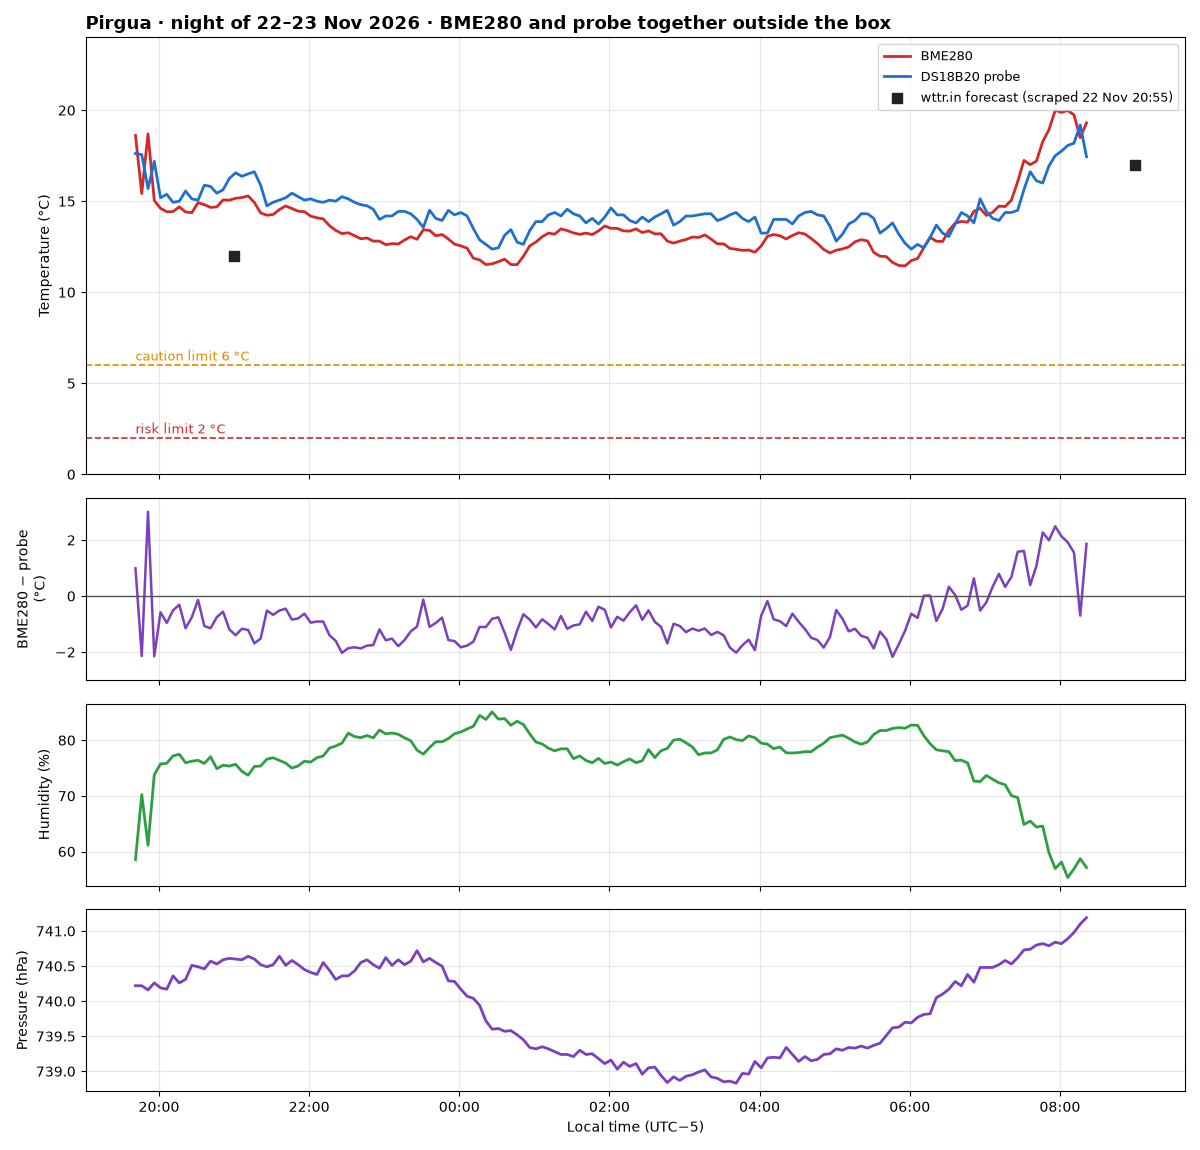
\includegraphics[width=\columnwidth]{night3.png}
\caption{Noche del 22 al 23 de noviembre de 2026 en Pirgua: BME280 y sonda juntos fuera de la caja, diferencia entre ambos, humedad y presi\'on. Los cuadrados negros son el pron\'ostico de wttr.in (en ingl\'es en la figura original).}
\label{fig:noche3}
\end{figure}

\begin{figure}[t]
\centering
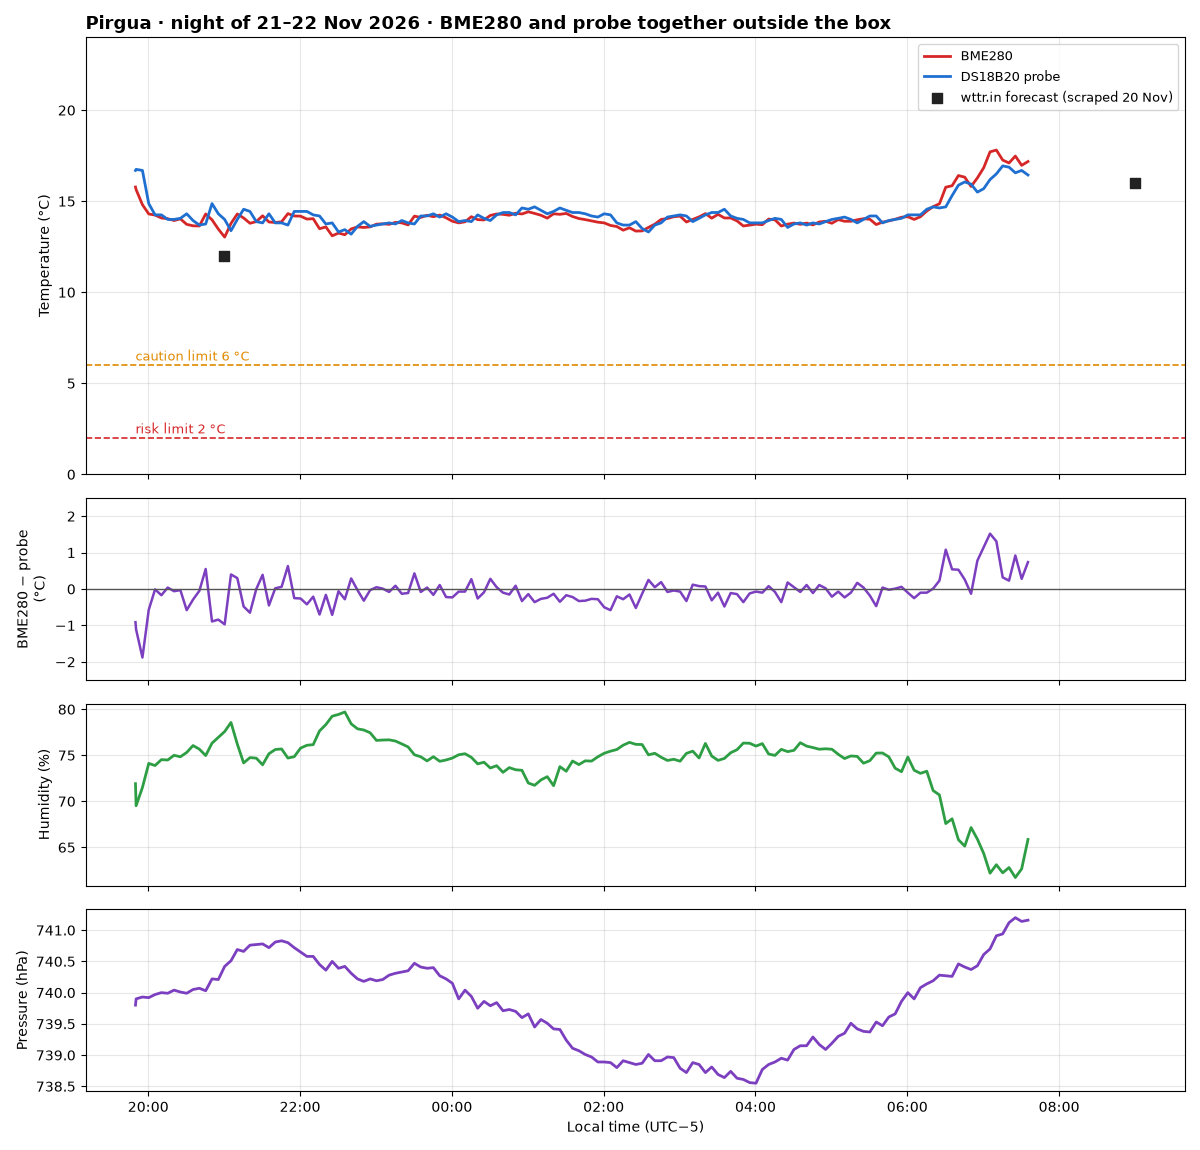
\includegraphics[width=\columnwidth]{night2.png}
\caption{Noche del 21 al 22 de noviembre de 2026, con la misma disposici\'on de la figura anterior.}
\label{fig:noche2}
\end{figure}

\subsection{Desfase entre el BME280 y la sonda}
En la segunda noche, entre las 21:00 y las 05:30, el BME280 menos la sonda dio $-0{,}12$\,$^\circ$C (desviaci\'on est\'andar 0,26\,$^\circ$C). Fue mayor cuando los sensores se adaptaban al aire exterior (primeros 40 minutos: $-0{,}53$\,$^\circ$C) y al amanecer (06:00 a 07:36: $+0{,}46$\,$^\circ$C, con picos de $+1{,}5$\,$^\circ$C), probablemente porque el sol llega a un sensor antes que al otro. En la tercera noche, con los mismos sensores, el desfase fue $-1{,}16$\,$^\circ$C (desviaci\'on est\'andar 0,46\,$^\circ$C) entre las 21:00 y las 05:00. El desfase no es constante, as\'i que no aplicamos ninguna correcci\'on. Las causas posibles, que no hemos comprobado, son una posici\'on distinta de los sensores dentro de la protecci\'on, un BME280 mojado (la humedad lleg\'o a 85\,\% y el aire estaba 2,4\,$^\circ$C sobre su punto de roc\'io) o un error de alguno de los dos sensores. No determinamos cu\'al de los dos sensores est\'a bien.

\subsection{Pron\'ostico frente a la medici\'on}
En las dos noches medidas, wttr.in dio 12\,$^\circ$C a las 21:00, mientras la sonda marcaba 14 y entre 15 y 16\,$^\circ$C. Son solo dos casos, pero el pron\'ostico parece subestimar la temperatura nocturna. El tablero (Fig.~\ref{fig:dash}) cuenta 21 coincidencias, 0 diferencias y 20 casos no comparables; las 21 coincidencias son triviales, porque el nodo con el modelo de prueba y el pron\'ostico dicen ``sin riesgo''. Una comparaci\'on significativa necesita una noche en que alguno de los dos prediga precauci\'on o riesgo.

\begin{figure}[t]
\centering
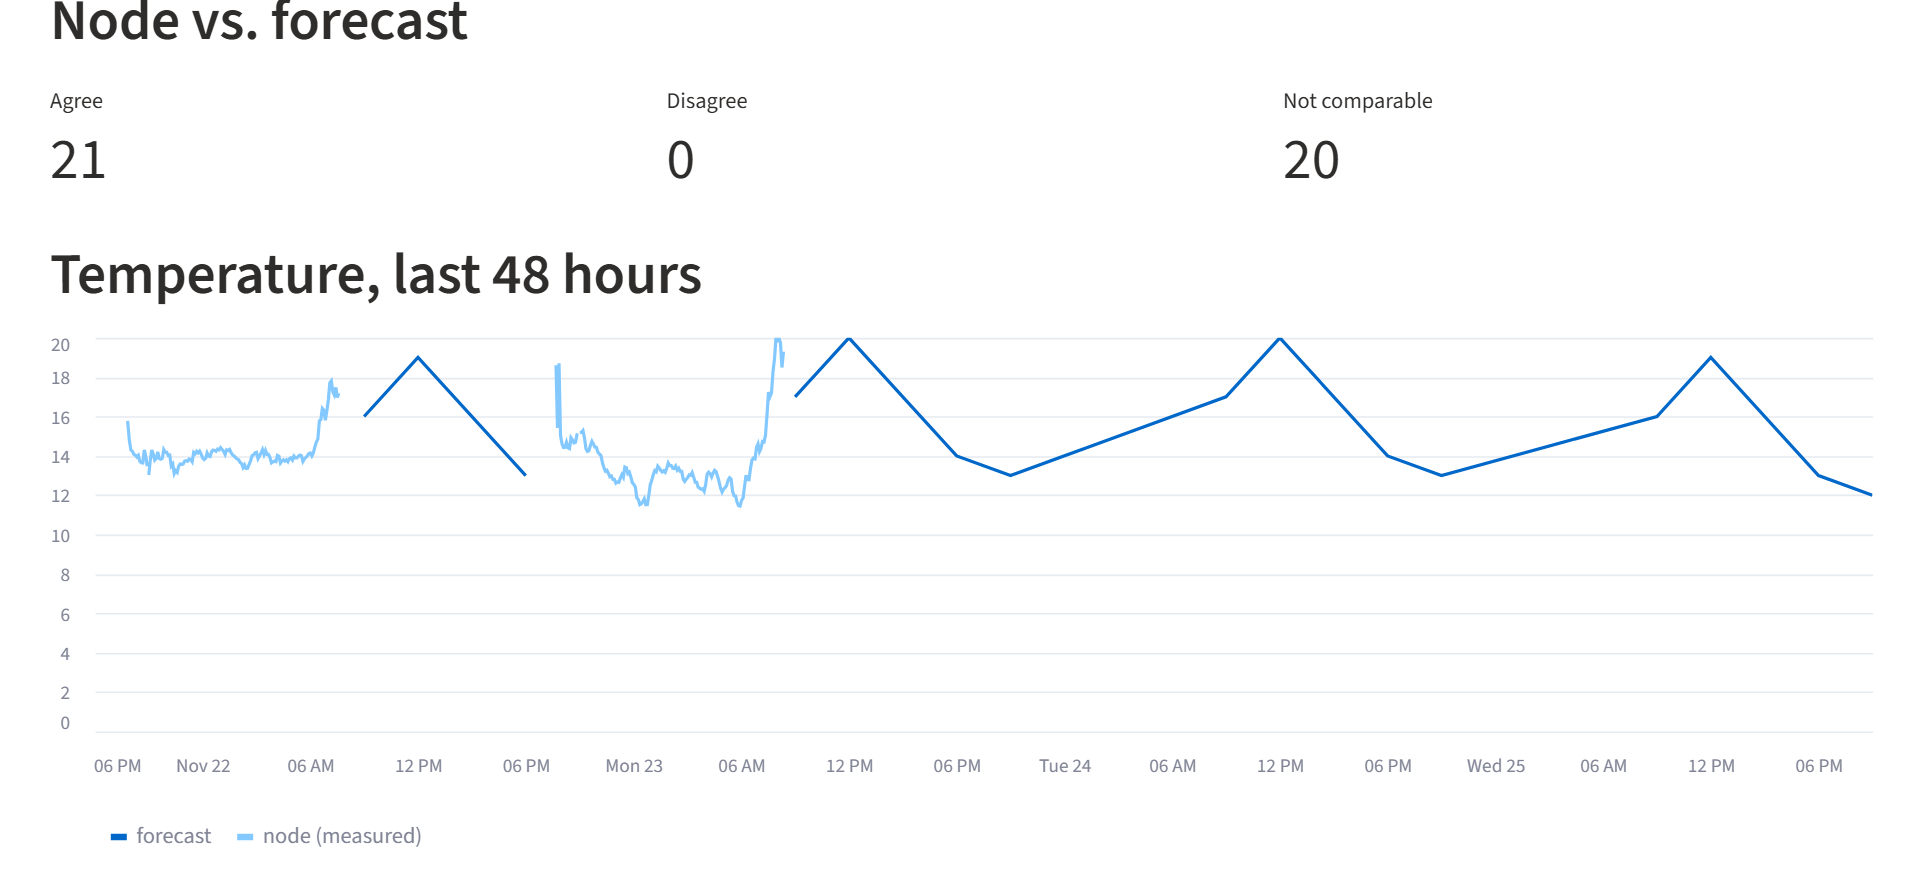
\includegraphics[width=\columnwidth]{dash.png}
\caption{Tablero: comparaci\'on nodo--pron\'ostico y temperatura de las \'ultimas 48 horas (interfaz en ingl\'es). Las lecturas y el pron\'ostico son reales; las predicciones vienen del modelo de prueba.}
\label{fig:dash}
\end{figure}

\subsection{Recursos del ESP32-S3 con el modelo final}
La Tabla~\ref{tab:recfinal} muestra el comando \texttt{BENCHMARK} del firmware con el modelo final, medido el 25 de noviembre de 2026 con la placa conectada al PC. Todo queda muy por debajo del 30\,\% que el curso usa como se\~nal para probar un dispositivo m\'as limitado: el tensor arena usa el 5,35\,\%, el programa el 2,84\,\% del flash y el pico de heap el 14,38\,\%. La mayor proporci\'on es la de la pila, con 29,15\,\%. Con una inferencia cada 30\,min, la carga de CPU es despreciable.

\begin{table}[t]
\caption{Recursos del ESP32-S3 con el modelo final (200 inferencias, 25 de noviembre de 2026)}
\label{tab:recfinal}
\centering
\small
\begin{tabular}{@{}>{\raggedright}p{2.6cm}>{\raggedright\arraybackslash}p{5cm}@{}}
\toprule
M\'etrica & Valor \\
\midrule
Latencia & 0,0528 $\pm$ 0,0138\,ms \\
Ciclos de CPU & 13\,509 por inferencia (240\,MHz) \\
Throughput & 18\,952 inferencias/s \\
Tensor arena & 876\,B (5,35\,\% de 16\,384\,B) \\
Modelo & 3\,160\,B (0,02\,\% de 16\,MB) \\
Programa & 476\,480\,B (2,84\,\% del flash; 36,35\,\% de la partici\'on) \\
Heap, pico & 52\,984 de 368\,408\,B (14,38\,\%) \\
Pila, pico & 2\,388 de 8\,192\,B (29,15\,\%) \\
Carga de CPU & 0,000003\,\% (una inferencia cada 30\,min) \\
Potencia & no medida \\
\bottomrule
\end{tabular}
\end{table}

\subsection{Comparaci\'on con la Pico (modelo de prueba)}
La Tabla~\ref{tab:rec} muestra la prueba en las dos placas con el mismo modelo de prueba (20 entradas, capas ocultas de 16 y 8 unidades, 2 clases), con ambas conectadas al PC y sin medir potencia. La latencia es la media de 200 ejecuciones. En la ESP32-S3 el uso de memoria y la latencia quedan muy por debajo del l\'imite del 30\,\% que sugiere el curso para probar una placa m\'as peque\~na. La Pico ejecut\'o el mismo modelo con una latencia de 0,087\,ms frente a 0,050\,ms, y la salida int8 de la ESP32-S3 coincidi\'o con la del PC en 100 de 100 vectores del modelo solo y en 50 de 50 ventanas completas.

\begin{table}[t]
\caption{Prueba de la cadena en las dos placas (modelo de prueba, 20 de noviembre de 2026)}
\label{tab:rec}
\centering
\small
\begin{tabular}{@{}>{\raggedright}p{1.9cm}>{\raggedright}p{2.9cm}>{\raggedright\arraybackslash}p{2.9cm}@{}}
\toprule
M\'etrica & ESP32-S3 (240\,MHz) & Pico (200\,MHz) \\
\midrule
Latencia (200 ejec.) & 0,0504 $\pm$ 0,0161\,ms & 0,0871 $\pm$ 0,0218\,ms \\
Tensor arena & 876\,B (5,35\,\% de 16\,384\,B) & 964\,B (5,88\,\% de 16\,384\,B) \\
Modelo & 3\,152\,B (0,02\,\% de 16\,MB) & 3\,152\,B (0,15\,\% de 2\,MB) \\
Programa & 2,84\,\% del flash (36,34\,\% de la partici\'on) & 7,43\,\% del flash \\
RAM & heap pico 14,20\,\% & heap en uso 0,97\,\% \\
Potencia & no medida & no medida \\
\bottomrule
\end{tabular}
\end{table}

Los dos programas no son equivalentes: el de la ESP32-S3 tambi\'en lee los sensores, guarda en flash y puede usar Wi-Fi, mientras el de la Pico solo ejecuta el benchmark. Las filas del modelo (latencia y tensor arena) se pueden comparar directamente; las de programa y RAM, con esa salvedad. Con el firmware actual en la ESP32-S3 (17 de noviembre), el pico de pila fue 30,86\,\% y el del heap 14,13\,\%. La carga de CPU se estima como la latencia media dividida por el periodo de 30\,min entre inferencias, no con las herramientas de perfilado del fabricante.

La comparaci\'on con la Pico no se repiti\'o con el modelo final. Las dos redes tienen la misma forma (20 entradas y capas de 16 y 8 unidades) y solo cambia la capa de salida, de 2 a 3 clases; en el ESP32-S3 el tensor arena qued\'o igual (876\,B) y la latencia pas\'o de 0,050 a 0,053\,ms. No medimos el consumo de energ\'ia ni la energ\'ia por inferencia en ninguna de las dos placas.

\section{Discusi\'on y limitaciones}
Lo que s\'i est\'a demostrado es que la cadena completa funciona: el nodo mide durante noches enteras sin PC, el firmware ejecuta el modelo int8 final y da la misma clase que el PC, el scraper y la tabla hash alimentan un tablero y el consumo de memoria y tiempo de la inferencia es peque\~no.

Lo que no est\'a demostrado es lo central del proyecto: que el nodo clasifique bien una helada. Faltan tres cosas. Primero, no hay noches fr\'ias en el conjunto propio, as\'i que la hip\'otesis de que Pirgua es m\'as fr\'io que la estaci\'on del IDEAM sigue sin probarse. Segundo, el modelo se entren\'o y se prob\'o solo con datos p\'ublicos; en el ESP32-S3 reproduce la clase del PC, pero eso no dice nada de su acierto en Pirgua. Tercero, el desfase entre sensores no es constante, as\'i que incluso con noches fr\'ias la incertidumbre de la medici\'on es del orden de un grado. Adem\'as, la fuente del pron\'ostico no cubre las horas del m\'inimo diario y solo tenemos dos comparaciones con ella. Si en toda la temporada el nodo no registra una noche bajo el umbral, lo reportaremos as\'i, porque entrenar y evaluar solo con datos p\'ublicos no responde la pregunta de investigaci\'on.

\section{Pruebas y reproducibilidad}
El repositorio incluye 46 pruebas autom\'aticas en Python y una prueba en C++ del buffer circular, que no necesitan placa, sensores ni red. Cubren la f\'ormula del punto de roc\'io, el relleno de vac\'ios cortos, el c\'alculo del m\'inimo de las pr\'oximas 6\,h, la partici\'on por d\'ias sin d\'ias compartidos, la tabla hash, el desfase entre sensores, la comparaci\'on nodo--pron\'ostico y el an\'alisis de la p\'agina del pron\'ostico. No cubren el entrenamiento ni la conversi\'on, porque necesitan un conjunto de datos real. Los archivos crudos del nodo nunca se editan: los periodos v\'alidos se declaran en la configuraci\'on y el script de preparaci\'on ignora el resto, de modo que las pruebas en interior y las lecturas del arranque no contaminan el conjunto. Las versiones del conjunto de datos se guardan sin sobrescribirse, junto con una copia de la configuraci\'on usada.

\section{Conclusiones y trabajo pendiente}
Se construy\'o y verific\'o la cadena de adquisici\'on, inferencia en el borde, scraping y comparaci\'on, con dos estructuras de datos propias de costo constante en promedio. El nodo midi\'o tres noches en Pirgua (dos v\'alidas) sin que la sonda bajara de 12,4\,$^\circ$C ni el BME280 de 11,45\,$^\circ$C, y por eso todav\'ia no se puede confirmar la hip\'otesis ni medir el acierto del modelo. El modelo de tres clases, entrenado con datos p\'ublicos, alcanz\'o un F1 promedio de 0,678 en punto flotante y 0,683 en int8. Cargado en el ESP32-S3, dio la misma clase que el PC en 100 de 100 vectores y en 50 de 50 ventanas crudas, con 0,053\,ms por inferencia y menos del 30\,\% de cada recurso. El consumo de energ\'ia no se midi\'o. Como trabajo futuro quedan medir el consumo, repetir la comparaci\'on con la Pico con el modelo final y capturar noches fr\'ias para validarlo en Pirgua.

\section*{Disponibilidad}
C\'odigo, datos crudos y documentaci\'on: \url{https://github.com/MahomerLeon/frost-node-tinyml}.

\begin{thebibliography}{00}
\bibitem{fao_frost} R. L. Snyder and J. P. de Melo-Abreu, \textit{Frost Protection: Fundamentals, Practice and Economics}, vol.~1, Environment and Natural Resources Series no.~10. Rome, Italy: FAO, 2005.
\bibitem{upra2024} IDEAM and UPRA, ``Cultivos y \'areas vulnerables a las heladas en enero de 2024,'' Bogot\'a, Colombia, 2024. [Online]. Available: \url{https://upra.gov.co/es-co/Documents/fenomeno_nino/20240125_Heladas-Enero-2024.pdf}
\bibitem{dane2020} DANE--SIPSA, ``Informe de mercados, semana del 8 al 14 de febrero de 2020,'' Bogot\'a, Colombia, Feb. 2020. [Online]. Available: \url{https://www.dane.gov.co/files/investigaciones/agropecuario/sipsa/heladas/informe-heladas-14-feb-2020.pdf}
\bibitem{ideam_data} IDEAM, ``Datos hidrometeorol\'ogicos crudos: temperatura, humedad y presi\'on, estaci\'on UPTC Tunja 2401500086,'' datos.gov.co, datasets sbwg-7ju4, uext-mhny and 62tk-nxj5. Accessed: Nov. 5, 2026.
\bibitem{diedrichs2018} A. L. Diedrichs, F. Bromberg, D. Dujovne, K. Brun-Laguna, and T. Watteyne, ``Prediction of frost events using machine learning and IoT sensing devices,'' \textit{IEEE Internet Things J.}, vol.~5, no.~6, pp.~4589--4597, 2018, doi: 10.1109/JIOT.2018.2867333.
% Referencia sin verificar (el DOI no se pudo comprobar): revisar antes de entregar.
\bibitem{calderon2026} E. Calder\'on Caro, D. A. Casta\~neda S\'anchez, J. R. Ballesteros, and J. W. Branch-Bedoya, ``Topoclimatic graph dataset for frost prediction in the tropical high-mountain Altiplano Cundiboyacense, Colombia,'' \textit{Data}, vol.~11, no.~8, Art. no.~205, 2026, doi: 10.3390/data11080205.
\bibitem{zenodo2026} E. Calder\'on Caro \textit{et al.}, ``Topoclimatic Graph Dataset for Frost Prediction,'' v1.0, Zenodo, 2026, doi: 10.5281/zenodo.20616866.
\bibitem{david2021} R. David \textit{et al.}, ``TensorFlow Lite Micro: Embedded machine learning for TinyML systems,'' in \textit{Proc. Mach. Learn. Syst. (MLSys)}, vol.~3, 2021, pp.~800--811.
\bibitem{jacob2018} B. Jacob \textit{et al.}, ``Quantization and training of neural networks for efficient integer-arithmetic-only inference,'' in \textit{Proc. IEEE Conf. Comput. Vis. Pattern Recognit. (CVPR)}, 2018, pp.~2704--2713.
\bibitem{banbury2020} C. R. Banbury \textit{et al.}, ``Benchmarking TinyML systems: Challenges and direction,'' arXiv:2003.04821, 2020.
\bibitem{alduchov1996} O. A. Alduchov and R. E. Eskridge, ``Improved Magnus form approximation of saturation vapor pressure,'' \textit{J. Appl. Meteorol.}, vol.~35, no.~4, pp.~601--609, 1996.
\bibitem{esp32s3} Espressif Systems, ``ESP32-S3 Series Datasheet.'' [Online]. Available: \url{https://www.espressif.com/sites/default/files/documentation/esp32-s3_datasheet_en.pdf}
\bibitem{rp2040} Raspberry Pi Ltd., ``RP2040 Datasheet.'' [Online]. Available: \url{https://datasheets.raspberrypi.com/rp2040/rp2040-datasheet.pdf}
\bibitem{bme280} Bosch Sensortec, ``BME280 Combined humidity and pressure sensor, Datasheet.''
\end{thebibliography}

\end{document}
